\chapter{Arquitectura de Spark}

El término “arquitectura” en informática remite a la estructura lógica y física de los componentes de una computadora. Si nos detenemos a estudiar la arquitectura de Spark, la primera característica identificativa es su uso de la conocida arquitectura maestro-esclavo o maestro-trabajador, que, como bien indica su terminología, consta de un nodo maestro y muchos nodos esclavos.\\
 
La arquitectura de Spark se compone de dos procesos: el driver y los executors[\ref{Arquitectura}]. Ambos serán descritos más adelante, pero aclaremos por ahora que el driver es el coordinador central, el cual se comunica con el cluster manager, encargado de orquestar los nodos esclavos, donde corren los executors y que, además, el driver y los executors se ejecutan en sus propios procesos de Java.\\
 
Para ir dibujando nuestra arquitectura necesitamos preguntarnos cómo se ponen en funcionamiento las aplicaciones en Spark. El proceso es el siguiente: Las aplicaciones de Spark se ejecutan como conjuntos de procesos independientes en un clúster, coordinados por el objeto SparkContext en su programa principal, el driver. Cuando ejecutamos Spark en un clúster, SparkContext se conecta al cluster manager, encargado de asignar recursos en el clúster. Una vez conectado, Spark adquiere executors en los nodos del clúster, que son procesos que ejecutan cúlculos y almacenan datos para su aplicación. A continuación, envía su código de aplicación (definido por archivos JAR o Python pasados a SparkContext) a los esclavos. Por último, SparkContext envía tareas a los esclavos para que se ejecuten.\\
 
Spark puede ejecutar varias aplicaciones en un clúster al mismo tiempo. Las aplicaciones están programadas por el administrador del clúster (cluster manager) y corresponden a un SparkContext. Cada aplicación obtiene sus propios agentes executors, que permanecen activos durante toda la aplicación y ejecutan tareas en varios subprocesos. Este hecho tiene la ventaja de aislar aplicaciones entre sí, tanto en el lado de la programación (cada driver programa sus propias tareas), como en el lado del executor (las tareas de diferentes aplicaciones se ejecutan en diferentes Máquinas Virtuales Java). Sin embargo, también significa que los datos no se pueden compartir en diferentes aplicaciones Spark sin escribirlo en un sistema de almacenamiento externo.\\
 
\section{Driver}
 
Como hemos señalado antes, el driver es el coordinador central, ya que un programa Spark se ejecuta en el nodo del driver y este envía instrucciones a los executors. Es un proceso JVM que ejecuta la función main() de la aplicación y crea el SparkContext para una aplicación de Spark. También aloja el DAG Scheduler y el Task Scheduler, de los que hablaremos no muy tarde.\\

El driver debe ser direccionable a través de la red desde los nodos esclavos, en tanto que es el que escucha y acepta las conexiones entrantes de sus executors a lo largo de su vida útil. Además, el driver es el encargado de traducir el código de usuario en un trabajo específico y de crear tareas convirtiendo aplicaciones en pequeñas unidades de ejecución.\\
 
\section{Executors}
 
Son agentes distribuidos responsables de la ejecución de las tareas, siendo ellos los que procesan los datos, los mantienen en memoria o los almacenan en disco.\\
 
Cada aplicación tiene sus propios executors. Los executor se ejecutan durante toda la vida de una aplicación de Spark. Pueden ejecutar múltiples tareas a lo largo de su vida, tanto de forma secuencial como paralela. Suelen ser de asignación estática. No obstante, en caso de que así lo requiramos, podemos configurarlos para hacer la asignación dinámica.\\
 
También informan de las métricas parciales mediante el uso del hilo del transmisor Heartbeat. Cuando un executor se inicia, se registra con el driver, comunicándose directamente con él para ejecutar tareas.\\
 
Sobre la ubicación de los executor, cabe señalar que residen en los nodos esclavos del clúster, que son cualquier nodo que pueda ejecutar código de aplicación en el clúster. Cada executor es su propia JVM, y un executor no puede abarcar múltiples nodos, aunque un nodo puede contener varios executors.\\
 
% AÑADIR NOTA A PIE DE PÁGINA ACERCA DE QUÉ SON LOS AGENTES
 
\section{SparkContext}
 
El SparkContext es una variable de entorno que configura los servicios internos y establece una conexión con un entorno de ejecución de Spark. Es decir, con el clúster.
Una vez que se crea un SparkContext, puede usarlo para crear RDD, acumuladores y variables broadcast, acceder a los servicios de Spark y ejecutar trabajos (hasta que se detenga SparkContext). Proporciona acceso al clúster a través del cluster manager.
SparkContext es esencialmente un cliente del entorno de ejecución de Spark y actúa como el maestro de su aplicación.\\

SparkContext determina cuántos recursos se asignan a cada executor. Como veremos más adelante, cuando se lanza un trabajo de Spark, cada executor tiene ranuras para ejecutar las tareas necesarias para calcular un RDD. De esta forma, podemos pensar en un SparkContext como un conjunto de parámetros de configuración para ejecutar trabajos de Spark. Estos parámetros (por ejemplo, la URL del nodo maestro) están expuestos en el objeto SparkConf, utilizado para crear un SparkContext.\\
 
\section{DAG Sheduler}
 
El DAGSheduler, a quien ya habíamos introducido, es el responsable de manejar la ejecución de una aplicación en Spark, dividiéndola en trabajos, etapas y tareas. Estos conceptos los estudiaremos detenidamente más adelante para así centrarnos a lo largo de este subapartado en comprender cómo actúa el DAGScheduler de Spark y por qué este comportamiento supone una mejora con respecto a otros sistemas.\\

Se trata de la capa de planificación de alto nivel \cite{05GitDAG} que implementa la programación orientada a la etapa. Lo hace calculando un DAG (directed aciclid graph) de etapas para cada trabajo, realizando un seguimiento de los RDD, a la par que busca un cronograma mínimo para ejecutar el trabajo. Por lo tanto, es el encargado de transformar un plan de ejecución lógico (es decir, el linaje de RDD de dependencias) en un plan de ejecución físico. Además de crear un DAG de etapas, DAGScheduler determina las ubicaciones más apropiadas para ejecutar cada tarea, teniendo en cuenta el estado actual de la memoria caché, evitando así recalcular RDD que hayan sido cacheados. También se ocupa de borrar las estructuras de datos una vez hayan finalizado las tareas que dependen de ellos, optimizando así el uso de memoria. Por último, bajo su responsabilidad está la recuperación ante fallas debidas a la pérdida de archivos durante el shuffle. Lo hace volviendo a computar las etapas afectadas en las particiones perdidas.\\

Este modelo es una generalización del modelo MapReduce, el cual crea un DAG con dos estados, Map y Reduce. El cambio de etapas en un DAG en Spark viene marcado por una transformación con dependencias wide, por lo tanto, puede canalizar transformaciones con dependencias narrow juntas, sin necesidad de escribir a disco entre cada una, obteniendo así un mejor rendimiento que el de MapReduce, que necesita escribir en disco los resultados entre las etapas Map y Reduce.\\

\begin{figure}[t]
	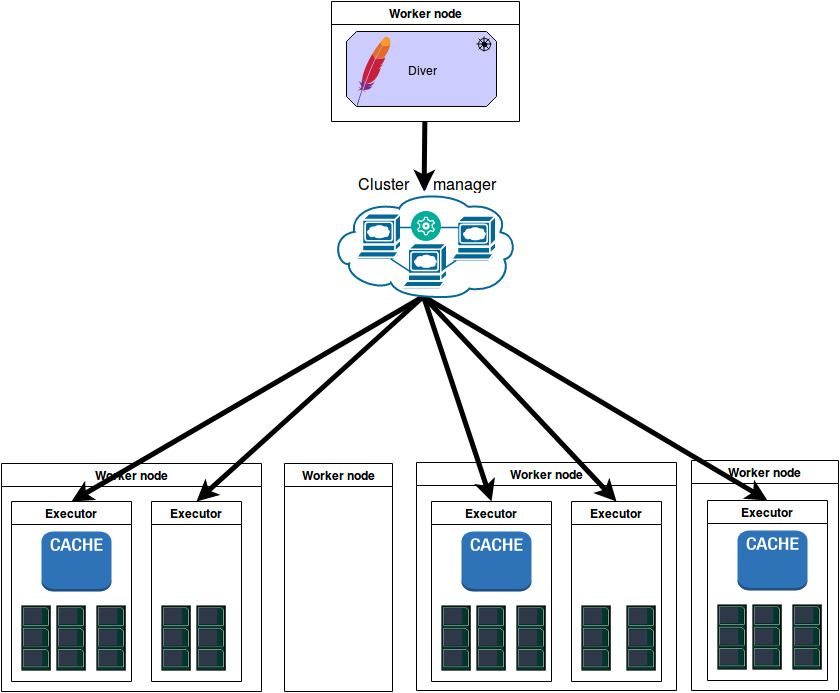
\includegraphics[scale=0.6]{img/arquitectura}
	\centering
	\caption{Arquitectura de Spark}
	\label{Arquitectura}
\end{figure}
